\documentclass[border=5mm]{standalone}
\usepackage{tkz-euclide}
\usetkzobj{all}

\begin{document}

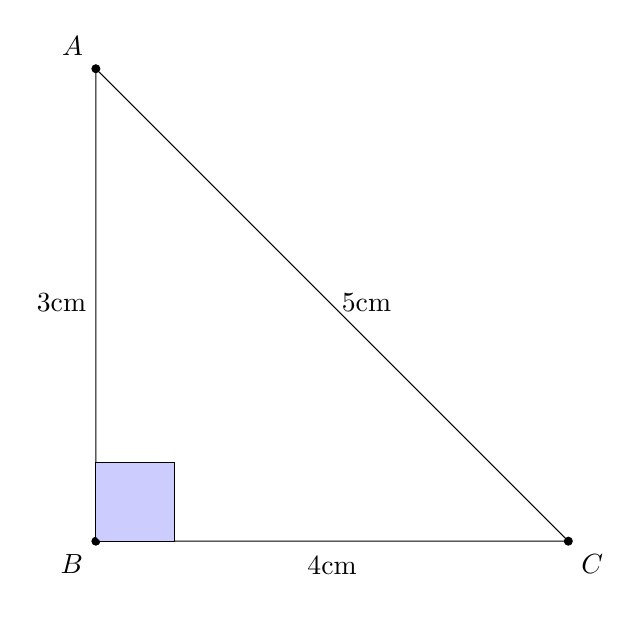
\begin{tikzpicture}
[
 scale=2,
  >=stealth,
  point/.style = {draw, circle, fill = black, inner sep = 1pt},
]

\node (B) at (0,0) [point,label = below left:$B$] {};
\node (A) at (0,3)[point,label = above left:$A$] {};
\node (C) at (3,0)[point,label = below right:$C$] {};
\draw (A) -- (B) -- (C) -- (A);

\tkzMarkRightAngle[fill=blue!20,size=0.5](A,B,C)

\node [left] at (0,1.5) {\strut 3cm};
\node [below] at (1.5,0) {\strut 4cm};
\node [right] at (1.5,1.5) {\strut 5cm};




\end{tikzpicture}

\end{document}